\documentclass{article}
\usepackage{pgfplots}
\usepackage{pgfplotstable}
\pgfplotsset{compat=1.17}

\begin{document}

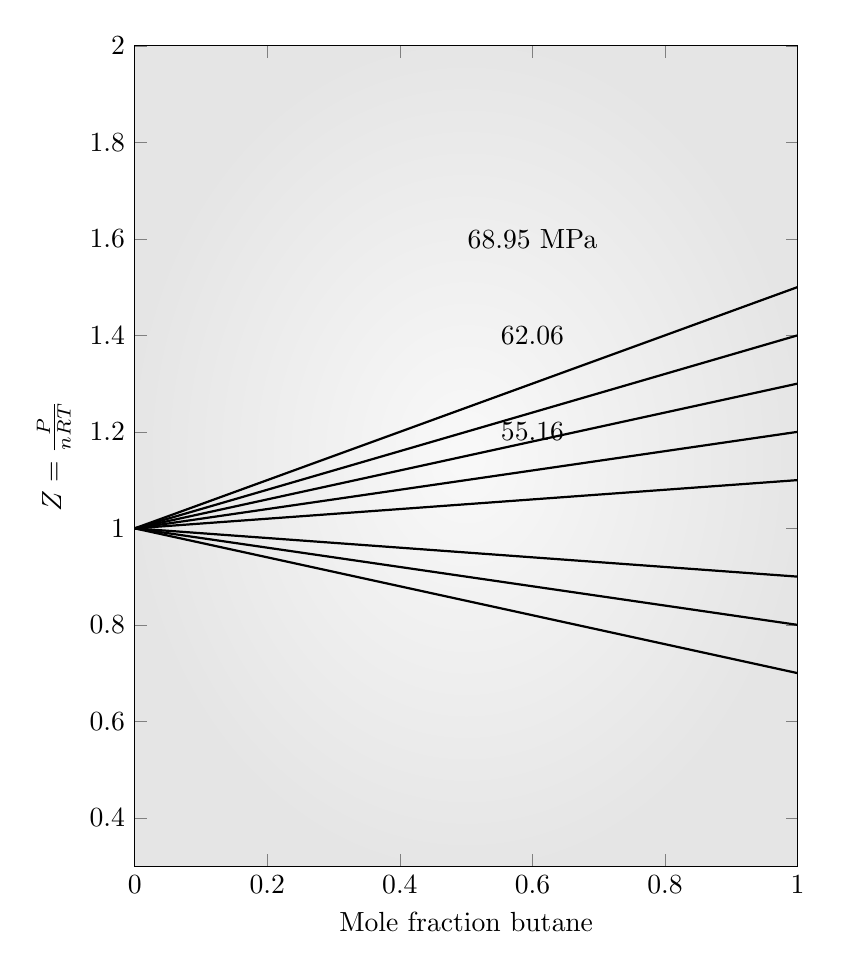
\begin{tikzpicture}
    \begin{axis}[
        width=10cm, height=12cm,
        xlabel={Mole fraction butane},
        ylabel={$Z = \frac{P}{nRT}$},
        xmin=0, xmax=1,
        ymin=0.3, ymax=2.0,
        domain=0:1,
        samples=50,
        axis background/.style={
            shading=radial, 
            inner color=gray!5, 
            outer color=gray!20
        }
    ]
    
    % Example curves
    \addplot[black, thick] {1.0 + 0.5*x};
    \addplot[black, thick] {1.0 + 0.4*x};
    \addplot[black, thick] {1.0 + 0.3*x};
    \addplot[black, thick] {1.0 + 0.2*x};
    \addplot[black, thick] {1.0 + 0.1*x};
    \addplot[black, thick] {1.0 - 0.1*x};
    \addplot[black, thick] {1.0 - 0.2*x};
    \addplot[black, thick] {1.0 - 0.3*x};

    % Labels (adjust as needed)
    \node at (axis cs:0.6,1.6) {68.95 MPa};
    \node at (axis cs:0.6,1.4) {62.06};
    \node at (axis cs:0.6,1.2) {55.16};

    \end{axis}
\end{tikzpicture}

\end{document}
